\documentclass{article}

\usepackage{amsmath, parskip, tikz}
\usetikzlibrary{automata}
\usetikzlibrary{positioning}
\usetikzlibrary{arrows}
\usepackage[margin=1.25in]{geometry}
\usepackage[shortlabels]{enumitem}

\renewcommand{\thesection}{\arabic{section}.}
\renewcommand{\thesubsection}{\alph{section}.}

\tikzset{
    node distance=2.5cm,
    every state/.append style={
        semithick,
        fill=gray!10
    },
    initial/.append style={
        initial text={},
        initial distance=0.5cm
    },
    accepting/.append style={
        double=gray!10,
        double distance=2pt,
        outer sep=1pt
    },
    every edge/.append style={
        draw,
        ->,>=stealth',
        auto,
        semithick
    }
}

\title{Homework 2: DFAs and NFAs}
\author{Will Griffin}

\begin{document}
    \maketitle

    \section{Divisibility Tests} 

    Define, for all $k > 0$,
    \begin{equation*}
        D_k = \{w \in \{0, \ldots, 9\}^* \mid w \text{ is the decimal representation of } k\}
    \end{equation*}
    where $\varepsilon$ is considered to represent the number 0. For example, the strings $\varepsilon$, \texttt{0}, \texttt{1234}, and \texttt{01234} all belong to $D_2$, but \texttt{99} and \texttt{099} do not.

    \begin{enumerate}[(\textasteriskcentered)]
        \item The DFA $D_2$ can be written as such:

            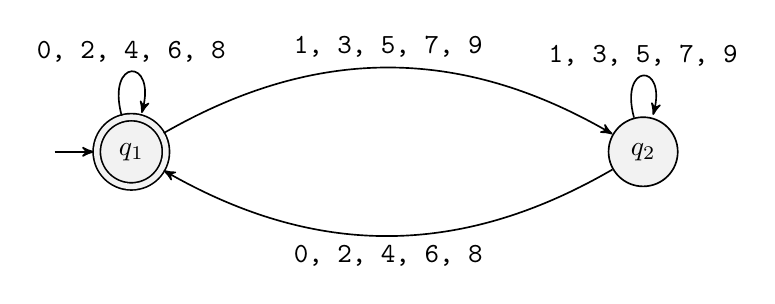
\begin{tikzpicture}
                \node[state, initial, accepting] (q1) {$q_1$};
                \node[state, right of=q1, xshift=4cm] (q2) {$q_2$};
                \draw (q1) edge[bend left] node {\texttt{1, 3, 5, 7, 9}} (q2)
                    edge[loop above] node {\texttt{0, 2, 4, 6, 8}} (q1);
                \draw (q2) edge[bend left] node {\texttt{0, 2, 4, 6, 8}} (q1)
                    edge[loop above] node {\texttt{1, 3, 5, 7, 9}} (q1);
            \end{tikzpicture}

        \item The DFA $D_3$ can be written as such:

            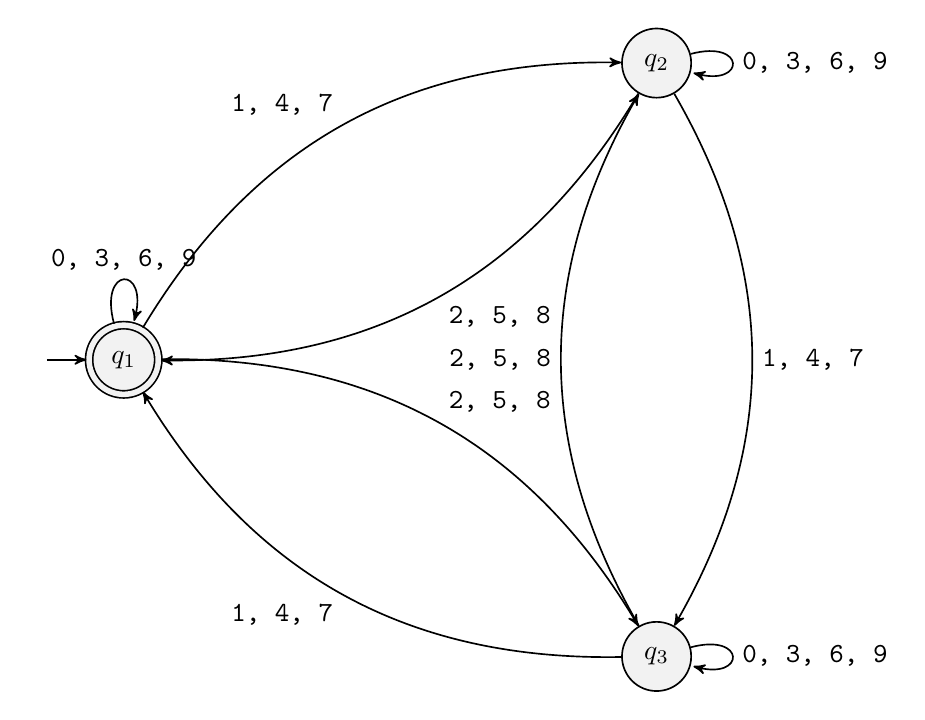
\begin{tikzpicture}
                \node[state, initial, accepting] (q1) {$q_1$};
                \node[state, above right of=q1, xshift=5cm, yshift=2cm] (q2) {$q_2$};
                \node[state, below right of=q1, xshift=5cm, yshift=-2cm] (q3) {$q_3$};
                \draw (q1) edge[loop above] node {\texttt{0, 3, 6, 9}} (q1)
                    edge[bend left] node {\texttt{1, 4, 7}} (q2)
                    edge[bend left] node {\texttt{2, 5, 8}} (q3);
                \draw (q2) edge[loop right] node {\texttt{0, 3, 6, 9}} (q2)
                    edge[bend left] node {\texttt{1, 4, 7}} (q3)
                    edge[bend left] node {\texttt{2, 5, 8}} (q1);
                \draw (q3) edge[loop right] node {\texttt{0, 3, 6, 9}} (q3)
                    edge[bend left] node {\texttt{1, 4, 7}} (q1)
                    edge[bend left] node {\texttt{2, 5, 8}} (q2);
            \end{tikzpicture}

        \item For any $k > 0$, the language $D_k$ is regular to the DFA $M = \left(Q, \Sigma, \delta, q_0, q_0\right)$ where
            \begin{itemize}
                \item $Q = \{q_0, \ldots, q_{k-1}\}$
                \item $\Sigma = \{0, \ldots, 9\}$
                \item $\delta (q_n, w \in \Sigma^*) = q_{(n \times 10 + w \pmod k)}$
            \end{itemize}
            For any $k > 0$, any whole number divided by $k$ has a remainder between $0$ and $k-1$. Therefore, the number of possible remainders for dividing a number by $k$ is equal to $k$, and thus the number of states for the DFA representing dividing a number by $k$ is equal to $k$. $Q$ is the set of all states of this DFA, where each state is numbered by the corresponding remainder ($Q = \{q_0, \ldots, q_{k-1}\}$). 

            By having each state correspond to a remainder, the DFA then stores the remainder of the number in the string $w \in \Sigma^*$ as each digit is processed. 

            Mathematically, the transition function $\delta$ operates as such on string $w \in \Sigma^*$: 
            \begin{enumerate}[(a)]
                \item Base Case ($w_1$):

                    The start state is $q_0$, so $r_{prev} = 0$. Therefore, $\delta (q_0, w_1) = q_{(0 \times 10 + w_1 \pmod k)} = q_{(w_1 \bmod k)}$

                \item Recursive Case ($w_i$, $0 < i \le |w|$):

                    The remainder of a number can be found through calculating the remainder of its digits one by one. If $N$ is the string of already read digits, and $d$ is the next digit, $N_{new} = N \times 10 + d$. Taking the modulus with respect to k, we obtain the remainder of $N_{new}$ calculated from the remainder of $N$:
                    
                    \begin{align*}
                        N_{new} \bmod k &= (N \times 10 + d) \bmod k \\
                        r_{new} &= (((N \bmod k)(10 \bmod k) \bmod k) + (d \bmod k)) \bmod k \footnotemark\\
                        r_{new} &= ((R \times (10 \bmod k) \bmod k) + (d \bmod k)) \bmod k \\
                        r_{new} &= (R \times 10 + d) \bmod k
                    \end{align*}

                    We can apply this to the transition function $\delta$, such that for a DFA at current state $q_j$, $j \in [0, k-1]$, processing symbol $w_i \in w$, $\delta (q_j, w_i) = q_{((j \times 10 + w_i) \bmod k)}$.

            \end{enumerate}

    \end{enumerate}

    \section{References}

    \begin{enumerate}[(1)]
        \item "Modulo/Properties." \textit{Wikipedia}, Wikimedia Foundation, 21 Jan. 2026, \\ \texttt{https://en.wikipedia.org/wiki/Modulo\#Properties\_(identities)}.
    \end{enumerate}
    
\end{document}
